\documentclass[onecolumn]{IEEEtran}
\IEEEoverridecommandlockouts
% The preceding line is only needed to identify funding in the first footnote. If that is unneeded, please comment it out.

\usepackage{cite}
\usepackage{amsmath,amssymb,amsfonts}
\usepackage{algorithmic}
\usepackage{graphicx}
\usepackage{textcomp}
\usepackage{xcolor}
\usepackage{amsmath,amsfonts,amsthm,amssymb}
\usepackage{setspace}
\usepackage{Tabbing}
\usepackage{enumitem}
\usepackage{fancyhdr}
\usepackage{lastpage}
\usepackage{extramarks}
\usepackage[hidelinks]{hyperref}
\usepackage{chngpage}
\usepackage{caption}
\usepackage{subcaption}
\usepackage{soul,color}
\usepackage{float}
\usepackage{graphicx,float,wrapfig}
\usepackage{titlesec}
\titleformat{\section}[hang]{\normalfont\large\bfseries}{\thesection}{1em}{}
% code listing settings
\usepackage{listings}
\lstset{
    language=Python,
    basicstyle=\ttfamily\small,
    aboveskip={1.0\baselineskip},
    belowskip={1.0\baselineskip},
    columns=fixed,
    extendedchars=true,
    breaklines=true,
    tabsize=4,
    prebreak=\raisebox{0ex}[0ex][0ex]{\ensuremath{\hookleftarrow}},
    frame=lines,
    showtabs=false,
    showspaces=false,
    showstringspaces=false,
    keywordstyle=\color[rgb]{0.627,0.126,0.941},
    commentstyle=\color[rgb]{0.133,0.545,0.133},
    stringstyle=\color[rgb]{01,0,0},
    numbers=left,
    numberstyle=\small,
    stepnumber=1,
    numbersep=10pt,
    captionpos=t,
    escapeinside={\%*}{*)}
}

\def\BibTeX{{\rm B\kern-.05em{\sc i\kern-.025em b}\kern-.08em
    T\kern-.1667em\lower.7ex\hbox{E}\kern-.125emX}}

% Add page numbers
\fancyhf{} % Clear all headers and footers
\fancyfoot[C]{\thepage} % Footer centered with page number
\renewcommand{\headrulewidth}{0pt} % Remove header rule
\renewcommand{\footrulewidth}{0pt} % Remove footer rule

%use this to compile without figures so I can mesure the length of the document
%\renewcommand{\includegraphics}[2][]{}

\pagestyle{fancy} % Enable fancy header/footer

\begin{document}
\title{ECE1512 Project B Report\\Part 1 - Mamba}

\author{\IEEEauthorblockN{Rémi Grzeczkowicz} \\
\IEEEauthorblockA{\textit{MScAC Student} \\
\textit{University of Toronto - Department of Computer Science}\\
Student Number: 1010905399\\
remigrz@cs.toronto.edu}
}

\maketitle
\thispagestyle{fancy} % Apply fancy header/footer, including the page number on the first page


% \begin{abstract}
% This document is a model and instructions for \LaTeX.
% This and the IEEEtran.cls file define the components of your paper [title, text, heads, etc.]. *CRITICAL: Do Not Use Symbols, Special Characters, Footnotes, 
% or Math in Paper Title or Abstract.
% \end{abstract}

% \begin{IEEEkeywords}
% component, formatting, style, styling, insert
% \end{IEEEkeywords}

%Table des matières centrée sur une nouvelle page
\section{Summary of the Mamba Model}
Mamba was introduced in \cite{gu2024mambalineartimesequencemodeling} with the goal of enhancing the performance of the Transformer model, particularly in language modeling tasks. The core idea behind Mamba is to replace the self-attention mechanism of the Transformer with a novel mechanism known as the \textit{Mamba mechanism}. This new approach can match the performance of the Transformer while significantly reducing both training and inference times. The architecture of Mamba is illustrated in Figure \ref{fig:mamba_architecture}.

\begin{figure}[H]
    \centering
    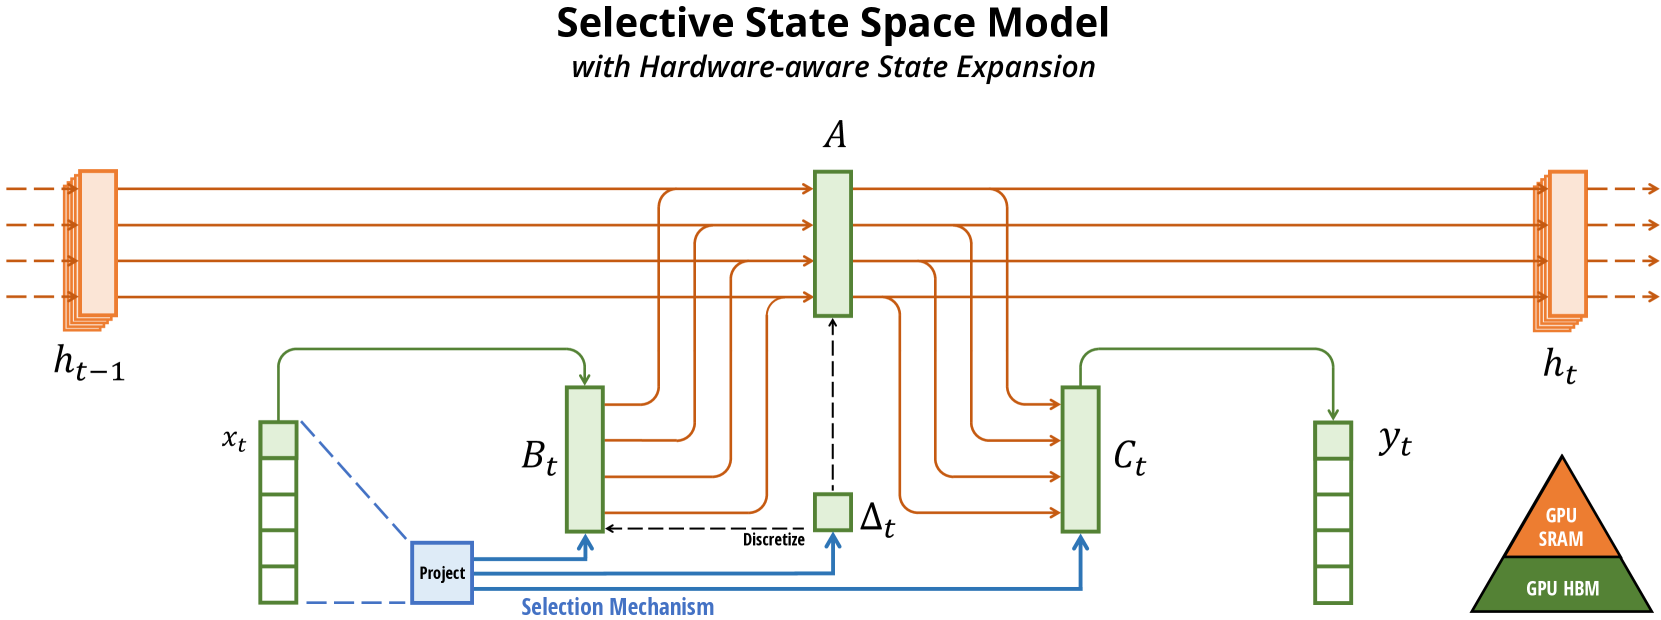
\includegraphics[width=0.8\textwidth]{images/mamba_architecture.png}
    \caption{Mamba architecture}
    \label{fig:mamba_architecture}
\end{figure}

\subsection{Mamba key ideas}
As previously mentioned, Mamba introduces a novel class of selective state-space models (SSMs) that address the inefficiencies of Transformers and prior subquadratic architectures for long-sequence tasks across various domains (language, audio, genomics). Its key ideas are as follows:
\begin{itemize}
    \item \textbf{Linear time complexity}: Mamba achieves linear time complexity with respect to sequence length during training, a significant improvement over the quadratic time complexity of the Transformer model. This mechanism also ensures constant time complexity during inference.
    \item \textbf{Selective mechanism}: The model incorporates input-dependent SSM parameters, enabling content-aware information propagation and dynamic filtering of irrelevant data. This selective mechanism mitigates the issues of vanishing and exploding gradients typically encountered by RNNs. Additionally, it enables the model to focus on relevant information, whereas RNNs are forced to propagate all information (or fail to do so if parameters are misconfigured).
    \item \textbf{Hardware-aware algorithm}: The algorithm is designed to minimize the number of transfer operations between CPU and GPU memory, which is often a bottleneck in various models, including Mamba.
    \item \textbf{Empirical success}: The Mamba model has been evaluated on tasks such as language modeling, DNA sequence modeling, and audio processing. It has either matched or outperformed previous state-of-the-art models in terms of performance, while offering significant speed improvements.
    \item \textbf{Open-source implementation}: Although not directly related to the model itself, the authors have released an open-source implementation of Mamba as a Python package available for installation via pip, with all the code provided on GitHub. This enables the scientific community to reproduce the results and integrate the model into their own projects.
\end{itemize}

\subsection{Technical contributions}
Mamba, through its technical implementation, offers several contributions to problems that were present in previous models:
\begin{itemize}
    \item \textbf{Input-Dependent SSMs}:
        \begin{itemize}
            \item Problem: Traditional Structured State Space Models (SSMs) are Linear Time Invariant (LTI), which makes them computationally efficient but unable to adapt to varying content, particularly in discrete or information-dense data like text.
            \item Solution: Mamba introduces a selection mechanism by making key parameters $\Delta$ (state update rate), $B$ (input projection), and $C$ (output projection) input-dependent. This allows the model to focus on relevant inputs while dynamically ignoring irrelevant ones. For example, in tasks like selective copying, the model selectively propagates relevant tokens, overcoming the LTI limitation.
            \item Impact: This mechanism enables Mamba to combine the expressiveness of Transformers with the efficiency of recurrent architectures.
        \end{itemize}
    \item \textbf{Efficient Scan Implementation}:
        \begin{itemize}
            \item Problem: The introduction of input-dependent parameters removes the time-invariance property, making traditional convolution-based computation methods inapplicable and increasing memory usage.
            \item Solution: Mamba employs a hardware-aware scan algorithm optimized for GPUs:
            \begin{itemize}
                \item \textbf{Kernel Fusion}: Reduces memory transfers between GPU levels by performing all operations within faster memory (e.g., SRAM). During backpropagation, intermediate states are recomputed instead of being stored, significantly reducing memory consumption.
                \item \textbf{Parallelized Scan}: Mamba implements a parallelized scan operation that avoids the sequential nature of traditional recurrent computations.
            \end{itemize}
            \item Impact: The model achieves true linear scaling, outperforming standard LTI convolutional implementations and even advanced Transformer optimizations (e.g., FlashAttention) for sequence lengths beyond 2k.
        \end{itemize}
    \item \textbf{Selection Mechanism}:
        \begin{itemize}
            \item \textbf{Dynamic Parameterization}: $\Delta$ controls how much to update or retain the state, functioning as a generalized RNN gate. Large $\Delta$ values reset the state to focus on new inputs, while small $\Delta$ values retain previous information.
            \item \textbf{Architectural Simplification}: $B$ and $C$ modulate the influence of input and state, respectively, providing fine-grained control over information flow. Mamba integrates these selective mechanisms into a single homogeneous block, eliminating the need for interleaved MLP or convolutional layers.
            \item \textbf{Generalization}: Mamba uses SiLU (Swish) activation for smooth gating and consistent performance. This mechanism is broadly applicable, enabling Mamba to adapt across diverse modalities such as language, genomics, and audio.
        \end{itemize}
\end{itemize}


\subsection{Areas of improvement}
Even though Mamba shows promise, there are still some areas for improvement that could be addressed in future work:
\begin{itemize}
    \item \textbf{Continuous-Discrete Spectrum}: Structured State Space Models (SSMs) were originally designed as discretizations of continuous systems, giving them a strong inductive bias for continuous-time data modalities such as audio or video signals. Mamba's selection mechanism, by introducing content dependency, improves performance on discrete data but could potentially hinder performance on continuous data, where LTI SSMs excel. Ablation studies on audio waveforms suggest that the selection mechanism may impair performance in such cases. Future research could explore ways to adapt the selection mechanism to better handle continuous data.
    \item \textbf{Downstream Applications}: While Mamba does not aim to encompass as many use cases as the ecosystem of Transformer-based foundation models, particularly LLMs, the latter provides a variety of features and interaction modes, such as fine-tuning, in-context learning, instruction tuning, quantization, and more. It remains to be seen whether Mamba possesses similar properties and affordances, and whether it can fully replace Transformers in those contexts.
    \item \textbf{Scaling}: Empirical evaluation of Mamba has been limited to small-scale models, below the threshold of most open-source LLMs like GPT-Neo and other recurrent models like RWKV, which have been evaluated at scales of 7 billion parameters and beyond. Whether Mamba remains competitive at such larger scales is yet to be determined. Scaling Mamba may also involve engineering challenges and model adjustments that have not been addressed in the current work.
\end{itemize}

\section{Accuracy improvement for translation}
Language modeling can be applied to various tasks, including translation. \cite{escolano2024residual} demonstrated that incorporating dropout into a model based on Transformers improves its BLEU score—a standard metric for evaluating translation quality—particularly in low-resource settings. This is because dropout acts as a regularization technique, helping the model generalize better and reduce overfitting. Building on this insight, we could explore integrating dropout into the Mamba model to evaluate its impact on performance. Given that Mamba has been utilized as a relatively small model in \cite{gu2024mambalineartimesequencemodeling}, this addition might enhance its generalization capabilities.

\subsection{New Architecture of Mamba}
The proposed architecture is shown in Figure \ref{fig:mamba_dropout}. Two layers of dropout are added to the Mamba model to prevent overfitting and improve generalization.


\begin{figure}[H]
    \centering
    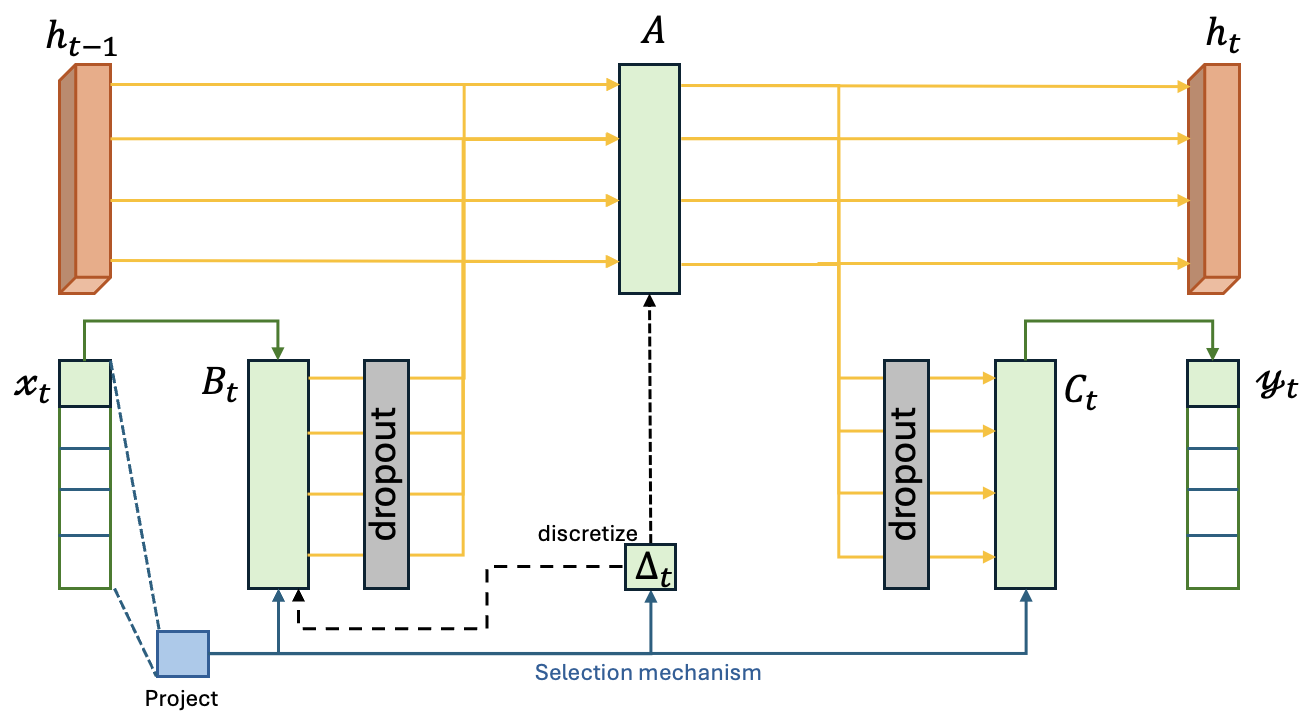
\includegraphics[width=0.8\textwidth]{images/mamba_architecture_dropout.png}
    \caption{Mamba architecture with dropout}
    \label{fig:mamba_dropout}
\end{figure}

\subsection{Experimental Setup}
To evaluate the impact of dropout on the Mamba model, we will run experiments on translation tasks and compare the results between the transformer encoder-decoder model, the transformer with dropout from \cite{escolano2024residual}, the original Mamba model, and the Mamba model with dropout. We will use the BLEU score as the evaluation metric.

For the dataset, we will use the Europarl dataset \cite{koehn2005europarl}, a parallel corpus of 21 languages. We will specifically use the English-French dataset for our experiments. Additionally, we will evaluate the model's generalization abilities by comparing translation performance between languages with similar origins (e.g., Germanic languages) and languages with different origins (e.g., Germanic and Slavic languages).

Furthermore, following the recommendation from \cite{pitorro2024effectivestatespacemodels}, we will ensure that the models are of similar size and complexity to allow for a fair comparison. Specifically, the models will have around 77M parameters to match the number of parameters in the transformer model \cite{pitorro2024effectivestatespacemodels}.

Finally, since dropout layers are generally more beneficial for smaller models \cite{escolano2024residual}, we will also evaluate the impact of dropout on the Mamba model at different sizes to determine if this effect persists across different model scales.

\section{Extension of the Mamba Model to Image Classification}
Transformers, through models like Vision Transformer (ViT) \cite{dosovitskiy2020image}, have shown great success in image classification tasks. \cite{khan2022transformers} also described a broader use of transformers. In the original work on Mamba, the model was tested on language modeling, DNA sequence modeling, and audio modeling tasks. We propose to extend the Mamba model to image classification tasks to evaluate its performance in this domain.

\subsection{Experimental Setup}
To evaluate performance on image classification, we propose running experiments on CIFAR-10 and CIFAR-100 \cite{alex2009learning}. Later, for technical reasons, we chose to use MedMamba \cite{yue2024medmamba} as the classifier. Since MedMamba was specifically developed to classify medical images, we will also test its performance on the MHIST dataset \cite{wei2021petri}. This dataset contains medical images and is more representative of the type of images that MedMamba was designed to classify. However, the authors of \cite{yue2024medmamba} did not evaluate the model on this dataset, making it an interesting case for assessing MedMamba's ability to generalize to other medical images, and more broadly to general images.

We will train the model on the CIFAR-10 and CIFAR-100 datasets and evaluate it on the test set for 500 epochs. We will use accuracy as the evaluation metric and compare the results with state-of-the-art models for image classification tasks. Additionally, we will evaluate the performance of the model on the MHIST dataset.

The code for the experiments is available on GitHub at \url{https://github.com/jacedoir/ECE1512_2024F_ProjectRepo_Grzeczkowicz} in the folder \textit{Project B/MedMamba}. The code is not modified from the original version provided by the authors of \cite{yue2024medmamba}.

\subsection{Results}

\begin{figure}[H]
    \centering
    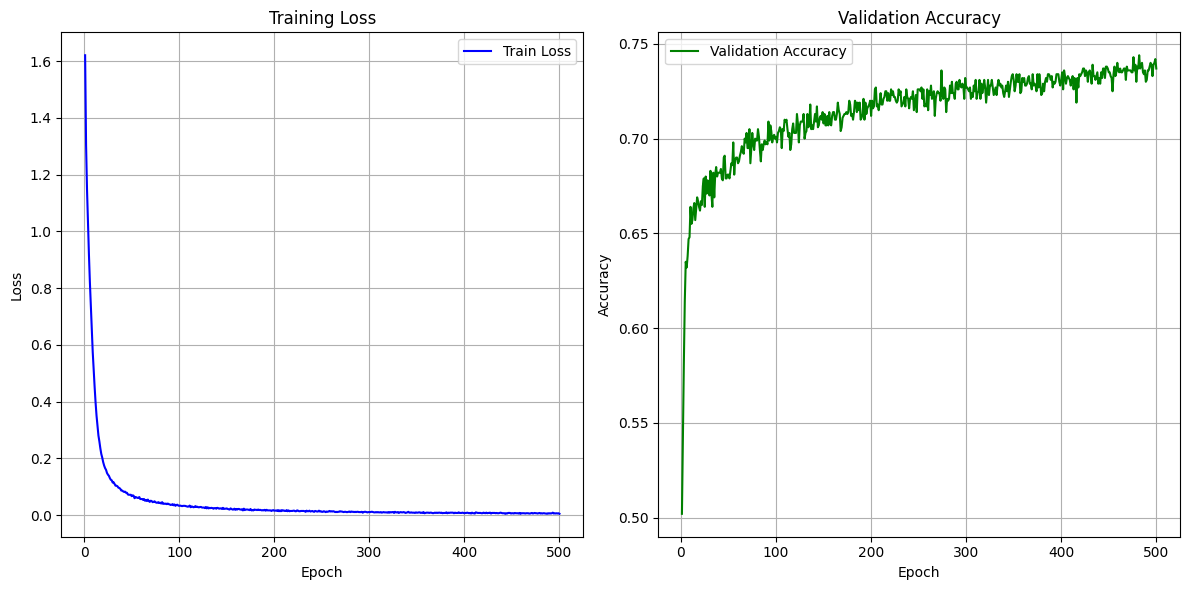
\includegraphics[width=0.8\textwidth]{images/cifar10.png}
    \caption{Results on CIFAR-10 dataset}
    \label{fig:cifar10}
\end{figure}
\begin{figure}[H]
    \centering
    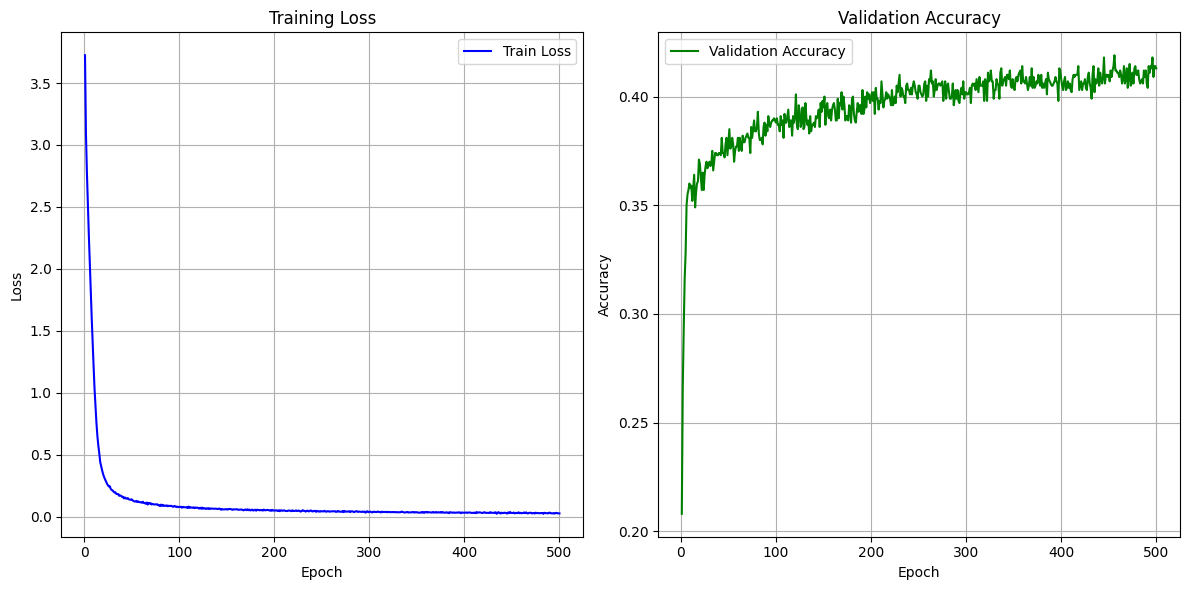
\includegraphics[width=0.8\textwidth]{images/cifar100.png}
    \caption{Results on CIFAR-100 dataset}
    \label{fig:cifar100}
\end{figure}
\begin{figure}[H]
    \centering
    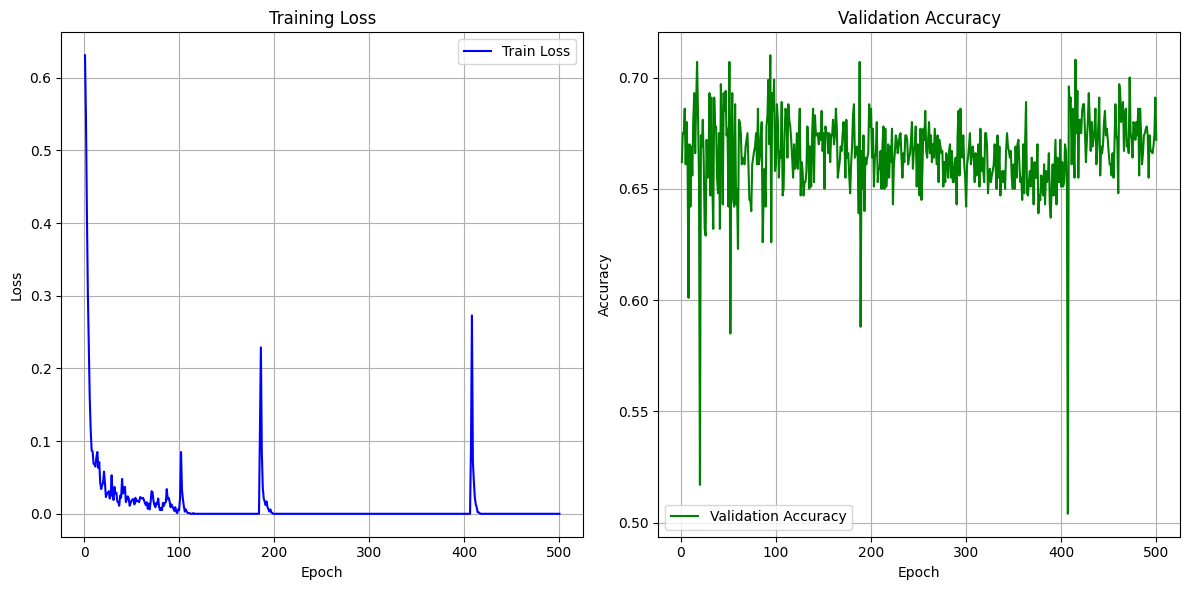
\includegraphics[width=0.8\textwidth]{images/MHIST.png}
    \caption{Results on MHIST dataset}
    \label{fig:mhist}
\end{figure}

The results of the experiments are not satisfactory. The model is unable to classify images correctly and underperforms compared to state-of-the-art models. Specifically, for CIFAR-10, the best accuracy achieved is 0.744, reached at epoch 481 (see Figure \ref{fig:cifar10}). According to \cite{paperswithcodePapersWithCifar10}, the best model, ViT-H/14 (Vision Transformer) \cite{dosovitskiy2020image}, achieves an accuracy of 0.995 after 14 epochs. For CIFAR-100, the best accuracy is 0.419, reached at epoch 455 (see Figure \ref{fig:cifar100}). According to \cite{paperswithcodePapersWithCifar100}, the best model is EffNet-L2 + SAM \cite{foret2020sharpness}, a model based on CNN developed by \cite{tan2019efficientnet} and enhanced by \cite{dosovitskiy2020image} using Sharpness-Aware Minimization, which achieves an accuracy of 0.9608. Finally, for the MHIST dataset, the best accuracy is 0.71, reached at epoch 93 (see Figure \ref{fig:mhist}). According to \cite{paperswithcodePapersWithMHIST}, the best model is MoCo-V2 \cite{foret2020sharpness}, which achieves an accuracy of 0.8803.

The difference in performance between the state-of-the-art models and MedMamba is smaller on the MHIST dataset, suggesting that the model may be more suited to medical images. However, it still underperforms, which could be due to the fact that Mamba may be interpreted as an RNN, and thus may require the data to be sequential, as is the case in domains like DNA, text, and audio. This is not true for image classification tasks, where data is typically not sequential. This discrepancy could explain why the model is underperforming on image classification tasks.

\section{Conclusion}
In this study, we explored the performance of the Mamba model in various domains, including language modeling, DNA sequence modeling, and image classification. While Mamba demonstrated promising results in sequential tasks, such as language and audio modeling, its performance on image classification tasks, including CIFAR-10, CIFAR-100, and MHIST, was suboptimal when compared to state-of-the-art models. The underperformance in image classification may be attributed to Mamba's inherent design, which is more suited for sequential data, as seen in its success with DNA, text, and audio data. The addition of dropout did not significantly improve the generalization capabilities of Mamba on these tasks.

Future work could focus on adapting the Mamba model to better handle image data, potentially by modifying its architecture to incorporate image-specific features or by investigating hybrid approaches that combine the strengths of both sequential and convolutional models. Additionally, further exploration into the scalability of Mamba at larger model sizes could provide insights into its performance on more complex datasets and tasks. Despite the challenges, the results presented here offer valuable insights into the potential applications of Mamba and highlight areas for improvement to enhance its applicability across diverse domains.


\bibliographystyle{plain}
\bibliography{mybibliography}
\end{document}
